\chapter{कार्बधात्विक उत्प्रेरण: मूल चरण और चक्र}\label{ch:b2:catalytic-cycles}

पैलेडियम लवण के कुछ मिलीग्राम किलोग्रामों अभिकर्मक वाले फ़्लास्क में दो \omterm{def:b2:huckel:aromatic}{ऐरोमैटिक}
वलयों को जोड़ सकते हैं: एक ही धातु परमाणु यह काम हज़ारों
बार करता है, हर चक्कर के बाद अपनी आरंभिक अवस्था में लौटते हुए। वह ऐसा कैसे करता है, यह
\omterm{def:b2:catalytic-cycles:cycle}{उत्प्रेरकी चक्र} बताता है, जो कुछ मूल चरणों का एक बंद अनुक्रम है।
चरणों के प्रकार थोड़े ही हैं, और हर एक धातु की ऑक्सीकरण अवस्था,
इलेक्ट्रॉन गणना और लिगैंडों की संख्या को एक निश्चित ढंग से बदलता है।
\cref{ch:b2:coordination-complexes} की इलेक्ट्रॉन गणना के साथ किसी चक्र को पढ़ा,
जाँचा, और कभी-कभी पूर्वानुमानित भी किया जा सकता है।

\begin{recall}
\Cref{ch:b2:coordination-complexes}: ऑक्सीकरण अवस्था, $d^n$, \omterm{def:b2:coordination-complexes:electron-count}{संयोजकता इलेक्ट्रॉन गणना},
\omterm{def:b2:coordination-complexes:electron-count}{18-इलेक्ट्रॉन नियम}, \omterm{def:b2:coordination-complexes:hapticity}{हैप्टिसिटी}। \Cref{ch:b2:ligand-field}: $\pi$-ग्राही लिगैंड और
\omterm{def:b2:ligand-field:pi-ligands}{पश्च-दान}। प्रथम वर्ष का खंड: उत्प्रेरक, समांगी उत्प्रेरण, मूल चरण,
दर-निर्धारक चरण, कार्बधात्विक यौगिक, ऑक्सीकरण संख्या।
\end{recall}

\begin{omfigure}
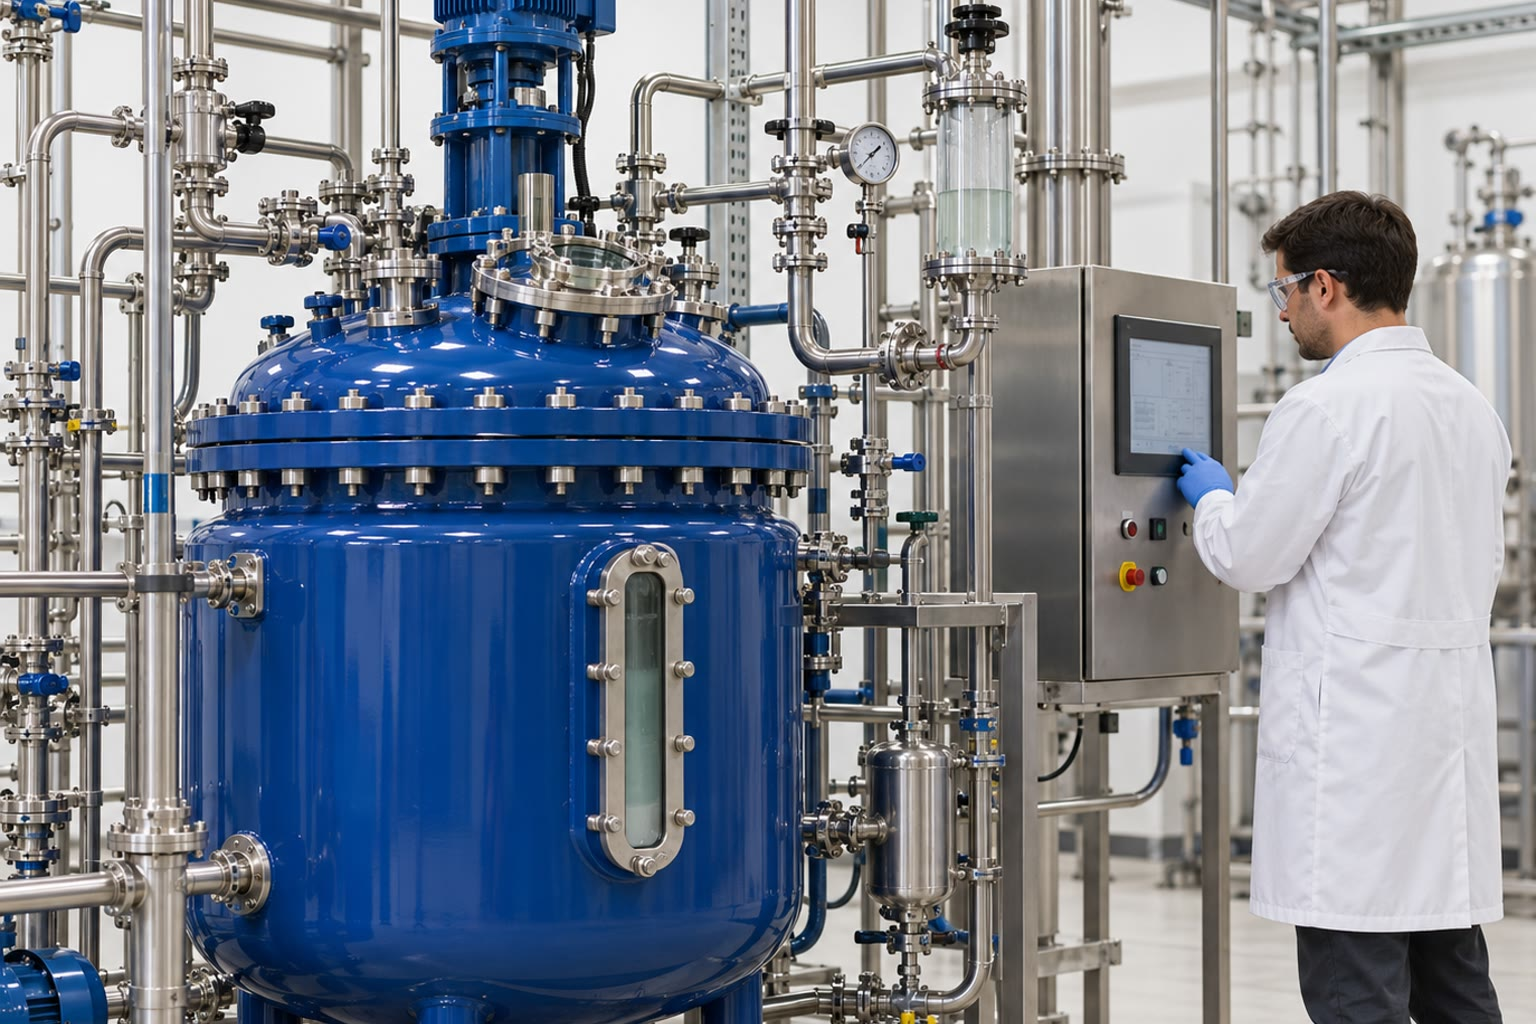
\includegraphics[width=0.62\linewidth]{images/book3/ai/b2-20-pilot-plant.jpg}

{\small प्रक्रम रसायन का एक प्रायोगिक संयंत्र: काँच-आस्तरित इस्पात का एक रिएक्टर, जिसमें
उत्पादन से पहले किसी उत्प्रेरित युग्मन को फ़्लास्क के पैमाने से बड़ा किया जाता है।}
\end{omfigure}

\section{कार्बधात्विक संकुलों की भाषा}

कार्बधात्विक संकुलों की गणना \cref{met:b2:coordination-complexes:electron-count} की तरह की जाती है,
कुछ और लिगैंडों के साथ: हाइड्राइड \ce{H-} और ऐल्किल या ऐरिल ऋणायन \ce{R-} हर एक दो
इलेक्ट्रॉन देते हैं और ऑक्सीकरण अवस्था में $-1$ गिने जाते हैं; \ce{CO}, फ़ॉस्फ़ीन \ce{PR3} और
$\eta^2$-ऐल्कीन दो इलेक्ट्रॉन देते हैं और 0 गिने जाते हैं; हैलाइड \ce{X-} दो देता है और
$-1$ गिना जाता है।

\begin{definition}[असंतृप्त संकुल]\label{def:b2:catalytic-cycles:unsaturated}
\emph{उपसहसंयोजी रूप से असंतृप्त संकुल}\index{उपसहसंयोजी रूप से असंतृप्त संकुल}
के 18 से कम संयोजकता इलेक्ट्रॉन होते हैं (प्रायः 16) और वह एक और लिगैंड बाँध सकता है: उसके पास
एक \emph{रिक्त स्थल}\index{रिक्त स्थल} होता है, अर्थात् उसके \omterm{def:b2:coordination-complexes:coordination-sphere}{उपसहसंयोजन मंडल} की एक स्थिति जो
किसी दो-इलेक्ट्रॉन दाता को ग्रहण करने के लिए मुक्त हो।
\end{definition}

रोडियम(I), इरिडियम(I), पैलेडियम(II) और
प्लैटिनम(II) के वर्ग समतलीय $d^8$ संकुल 16-इलेक्ट्रॉन संकुल हैं; पैलेडियम(0) बिसफ़ॉस्फ़ीनों \ce{PdL2} के 14 हैं।
ऐसे संकुल अधिकांश \omterm{def:b2:catalytic-cycles:cycle}{उत्प्रेरकी चक्रों} की सक्रिय स्पीशीज़ हैं।

\begin{method}[कार्बधात्विक संकुल की गणना]\label{met:b2:catalytic-cycles:count-organometallic}
\begin{enumerate}
  \item लिगैंडों की सूची बनाइए: ऋणायनी (\ce{H-}, \ce{R-}, \ce{X-}, \ce{C5H5-}) और उदासीन
        (\ce{CO}, \ce{PR3}, ऐल्कीन, विलायक)।
  \item ऑक्सीकरण अवस्था = संकुल का आवेश $-$ ऋणायनी लिगैंडों के आवेशों का योग।
  \item $n = g -$ ऑक्सीकरण अवस्था; गणना = $n + 2 \times$(दो-इलेक्ट्रॉन दाताओं की संख्या)
        $+$ हर $\eta^5$-\ce{C5H5-} के लिए 6।
  \item उपसहसंयोजन संख्या = घिरी हुई लिगैंड स्थितियों की संख्या।
\end{enumerate}
\end{method}

\section{लिगैंड विनिमय, ऑक्सीकारी योग, अपचायी विलोपन}

\begin{definition}[लिगैंड विनिमय]\label{def:b2:catalytic-cycles:ligand-exchange}
\emph{लिगैंड विनिमय}\index{लिगैंड विनिमय} वह मूल चरण है जिसमें \omterm{def:b2:coordination-complexes:coordination-sphere}{उपसहसंयोजन मंडल} का
एक लिगैंड दूसरे से प्रतिस्थापित होता है; यह न ऑक्सीकरण अवस्था बदलता है
और न, कुल मिलाकर, इलेक्ट्रॉन गणना। इसकी क्रियाविधियों का अध्ययन तृतीय वर्ष के खंड में है।
\end{definition}

\begin{definition}[ऑक्सीकारी योग और अपचायी विलोपन]\label{def:b2:catalytic-cycles:oxidative-addition}
\emph{ऑक्सीकारी योग}\index{ऑक्सीकारी योग} में कोई अणु A--B अपना A--B आबंध तोड़कर और
M--A तथा M--B आबंध बनाकर किसी धातु केंद्र से जुड़ता है।
\emph{अपचायी विलोपन}\index{अपचायी विलोपन} उलटा चरण है: एक-दूसरे के cis स्थित दो
लिगैंड A और B जुड़कर A--B बनाते हैं और धातु को छोड़ देते हैं।
\end{definition}

\begin{proposition}[ऑक्सीकारी योग की गणना]\label{prop:b2:catalytic-cycles:oa}
\omterm{def:b2:catalytic-cycles:oxidative-addition}{ऑक्सीकारी योग} धातु की ऑक्सीकरण अवस्था को 2, उसकी \omterm{def:b2:coordination-complexes:electron-count}{संयोजकता इलेक्ट्रॉन
गणना} को 2 और उसकी उपसहसंयोजन संख्या को 2 बढ़ाता है; \omterm{def:b2:catalytic-cycles:oxidative-addition}{अपचायी विलोपन} हर एक को 2 घटाता है।
\end{proposition}

\begin{proof}
बँध जाने के बाद A और B ऋणायन (\ce{H-}, \ce{R-}, \ce{X-}) गिने जाते हैं: दो नए ऋणायनी
लिगैंड ऑक्सीकरण अवस्था को 2 बढ़ाते हैं और $n$ को 2 घटाते हैं; वे दो युग्म देते हैं, $+4$
इलेक्ट्रॉन; गणना $-2 + 4 = +2$ से बदलती है। दो स्थितियाँ नई घिरती हैं।
उलटा चरण हर परिवर्तन को उलट देता है।
\end{proof}

\begin{example}[वास्का संकुल]\label{ex:b2:catalytic-cycles:vaska}
\ce{[IrCl(CO)(PPh3)2]}, वर्ग समतलीय: इरिडियम(I), $d^8$, 16 इलेक्ट्रॉन, चतुःउपसहसंयोजी।
यह डाइहाइड्रोजन जोड़ता है: \ce{[IrH2Cl(CO)(PPh3)2]}, इरिडियम(III), $d^6$, 18 इलेक्ट्रॉन, अष्टफलकीय,
दोनों हाइड्राइड cis।
\end{example}

\section{निवेशन, विलोपन, पारधात्वन}

\begin{definition}[निवेशन और $\beta$-हाइड्राइड विलोपन]\label{def:b2:catalytic-cycles:insertion}
\emph{प्रवासी निवेशन}\index{प्रवासी निवेशन} में धातु से बँधा कोई असंतृप्त लिगैंड
(ऐल्कीन, \ce{CO}) किसी cis M--H या M--C आबंध में निविष्ट होता है: \ce{M-H} और कोई
ऐल्कीन एक ऐल्किल \ce{M-CH2-CH2-H} देते हैं; \ce{M-R} और \ce{CO} एक ऐसिल \ce{M-C(=O)R} देते हैं।
\emph{$\beta$-हाइड्राइड विलोपन}\index{बीटा-हाइड्राइड विलोपन@$\beta$-हाइड्राइड विलोपन}
ऐल्कीन निवेशन का उलटा है: धातु के सापेक्ष $\beta$ कार्बन पर स्थित कोई हाइड्रोजन
धातु पर चला जाता है, और एक ऐल्कीन मुक्त होती है।
\end{definition}

\begin{proposition}[निवेशन की गणना]\label{prop:b2:catalytic-cycles:insertion}
\omterm{def:b2:catalytic-cycles:insertion}{प्रवासी निवेशन} ऑक्सीकरण अवस्था को बनाए रखता है और इलेक्ट्रॉन गणना को 2 घटाता है
(एक लिगैंड स्थिति मुक्त होती है); $\beta$-हाइड्राइड विलोपन गणना को 2 बढ़ाता है।
\end{proposition}

\begin{proof}
पहले: \ce{H-} (या \ce{R-}, ऋणायनी) और ऐल्कीन (उदासीन), दो लिगैंड, चार इलेक्ट्रॉन।
बाद में: एक ऐल्किल (ऋणायनी), दो इलेक्ट्रॉन। ऋणायनी आवेश अपरिवर्तित है: वही
ऑक्सीकरण अवस्था; दो इलेक्ट्रॉन और एक स्थिति खोई गई।
\end{proof}

\begin{proposition}[$\beta$-हाइड्राइड विलोपन की शर्तें]\label{prop:b2:catalytic-cycles:beta-h}
कोई धातु ऐल्किल $\beta$-हाइड्राइड विलोपन तभी करता है जब ऐल्किल के
$\beta$ कार्बन पर हाइड्रोजन हो और धातु के पास ऐल्किल के cis कोई \omterm{def:b2:catalytic-cycles:unsaturated}{रिक्त स्थल} हो।
\end{proposition}

\begin{proof}[तर्क]
चरण एक चतुःसदस्यी व्यवस्था M--C$_\alpha$--C$_\beta$--H से होकर जाता है जिसमें
हाइड्रोजन धातु तक पहुँचता है: इसके लिए वह हाइड्रोजन चाहिए, और ऐल्किल के बगल में उसे ग्रहण करने के लिए
एक खाली स्थिति। मेथिल, बेन्ज़िल, नियोपेंटिल और ऐरिल समूह, जिनके पास धातु तक पहुँच सकने वाला कोई $\beta$ हाइड्रोजन
नहीं है, इसके प्रति स्थायी हैं।
\end{proof}

\begin{definition}[पारधात्वन]\label{def:b2:catalytic-cycles:transmetalation}
\emph{पारधात्वन}\index{पारधात्वन} किसी कार्बनिक समूह को एक धातु
(या उपधातु: बोरॉन, जस्ता, टिन) से दूसरी धातु पर स्थानांतरित करता है, प्रायः किसी हैलाइड के बदले में।
\end{definition}

\begin{omfigure}
\begin{tikzpicture}[font=\small, >={Stealth}]
  \tikzset{omstepar/.style={->, thick}}
  \foreach \y/\l/\r/\top/\bot/\rev in {
      0/{$\mathrm{L}_n\mathrm{M}$}/{$\mathrm{L}_n\mathrm{M(A)(B)}$}/{+ A--B}/{ऑक्सीकारी योग}/{अपचायी विलोपन},
      -1.5/{$\mathrm{L}_n\mathrm{M(H)(CH_2{=}CH_2)}$}/{$\mathrm{L}_n\mathrm{M{-}CH_2CH_3}$}/{}/{प्रवासी निवेशन}/{$\beta$-हाइड्राइड विलोपन},
      -3.0/{$\mathrm{L}_n\mathrm{M(X)(R)}$}/{$\mathrm{L}_n\mathrm{M(R)(R')}$}/{+ R$'$--[B], $-$ X--[B]}/{पारधात्वन}/{},
      -4.5/{$\mathrm{L}_n\mathrm{M(X)}$}/{$\mathrm{L}_n\mathrm{M(X)(L')}$}/{+ L$'$}/{लिगैंड विनिमय या बंधन}/{}} {
    \node[cyclenode, anchor=east] (l) at (0,\y) {\l};
    \node[cyclenode, anchor=west] (r) at (5.2,\y) {\r};
    \draw[omstepar] ($(l.east)+(0.1,0.08)$) -- ($(r.west)+(-0.1,0.08)$) node[midway, above, font=\scriptsize] {\top};
    \node[font=\scriptsize, anchor=north] at (2.6,\y-0.02) {\bot};
    \node[font=\scriptsize, black!55, anchor=west] at (5.2,\y-0.5) {\rev};
  }
\end{tikzpicture}

{\small कार्बधात्विक उत्प्रेरण के मूल चरण। \omterm{def:b2:catalytic-cycles:oxidative-addition}{ऑक्सीकारी योग}: ऑक्सीकरण
अवस्था, गणना और उपसहसंयोजन संख्या $+2$; \omterm{def:b2:catalytic-cycles:oxidative-addition}{अपचायी विलोपन}: $-2$। \omterm{def:b2:catalytic-cycles:insertion}{प्रवासी
निवेशन}: गणना $-2$, ऑक्सीकरण अवस्था अपरिवर्तित; $\beta$-हाइड्राइड विलोपन: इसका
उलटा। \omterm{def:b2:catalytic-cycles:transmetalation}{पारधात्वन}: कोई कार्बनिक समूह बोरॉन, जस्ते या टिन से धातु पर जाता है।}
\end{omfigure}

\section{उत्प्रेरकी चक्र को पढ़ना}

\begin{definition}[उत्प्रेरकी चक्र]\label{def:b2:catalytic-cycles:cycle}
\emph{उत्प्रेरकी चक्र}\index{उत्प्रेरकी चक्र} मूल चरणों का वह बंद अनुक्रम है
जो अभिकर्मकों का उपभोग करता है, उत्पाद मुक्त करता है और अपने पहले संकुल का पुनर्जनन करता है।
अभिक्रिया में मिलाया गया वह यौगिक, जो चक्र के पहले संकुल में बदल जाता है,
\emph{पूर्व-उत्प्रेरक}\index{पूर्व-उत्प्रेरक} है। \emph{आवर्त संख्या}\index{आवर्त संख्या}
(TON) उत्प्रेरक की प्रति मात्रा बने उत्पाद की मात्रा है; \emph{आवर्त
आवृत्ति}\index{आवर्त आवृत्ति} (TOF) प्रति इकाई समय आवर्त संख्या है।
\end{definition}

\begin{proposition}[समग्र समीकरण]\label{prop:b2:catalytic-cycles:cycle-sum}
किसी \omterm{def:b2:catalytic-cycles:cycle}{उत्प्रेरकी चक्र} के चरणों का योग उत्प्रेरित अभिक्रिया का समीकरण है:
हर धातु संकुल एक बार उत्पाद के रूप में और एक बार अभिकारक के रूप में आता है, और कट जाता है।
\end{proposition}

\begin{proof}
चक्र बंद होने से हर मध्यवर्ती एक चरण द्वारा बनता है और अगले द्वारा उपभुक्त होता है;
चरणों को जोड़ने पर ये स्पीशीज़ दोनों ओर आती हैं और कट जाती हैं। जो बचती हैं वे
स्पीशीज़ हैं जो बाहर से प्रवेश करती हैं (अभिकर्मक) और बाहर निकलती हैं (उत्पाद)।
\end{proof}

\begin{method}[चक्र को पढ़ना]\label{met:b2:catalytic-cycles:read-cycle}
\begin{enumerate}
  \item हर संकुल के लिए ऑक्सीकरण अवस्था, इलेक्ट्रॉन गणना और
        उपसहसंयोजन संख्या परिकलित कीजिए।
  \item परिवर्तनों से हर चरण का नाम पहचानिए ($+2/+2/+2$: \omterm{def:b2:catalytic-cycles:oxidative-addition}{ऑक्सीकारी योग}; नियत ऑक्सीकरण अवस्था पर
        गणना $-2$: निवेशन; इत्यादि)।
  \item जाँचिए कि कोई संकुल 18 इलेक्ट्रॉनों से आगे न जाए और \omterm{def:b2:catalytic-cycles:unsaturated}{रिक्त स्थल} माँगने वाला चरण
        किसी असंतृप्त संकुल से आरंभ हो।
  \item चरणों को जोड़िए: योग समग्र समीकरण होना चाहिए।
\end{enumerate}
\end{method}

\begin{omfigure}
\begin{tikzpicture}[font=\small, >={Stealth}]
  \node[cyclenode] (n1) at (90:2.3) {\ce{[RhCl(PPh3)2]}\\ Rh(I), 14 e};
  \node[cyclenode] (n2) at (0:3.4) {\ce{[RhH2Cl(PPh3)2]}\\ Rh(III), 16 e};
  \node[cyclenode] (n3) at (270:2.3) {\ce{[RhH2Cl(PPh3)2(RCH=CH2)]}\\ Rh(III), 18 e};
  \node[cyclenode] (n4) at (180:3.4) {\ce{[RhH(CH2CH2R)Cl(PPh3)2]}\\ Rh(III), 16 e};
  \draw[cyclearc] (n1) to[bend left=20] node[cyclelabel, below left] {ऑक्सीकारी\\ योग} (n2);
  \draw[cyclearc] (n2) to[bend left=20] node[cyclelabel, left=12pt] {ऐल्कीन\\ बंधन} (n3);
  \draw[cyclearc] (n3) to[bend left=20] node[cyclelabel, above right] {प्रवासी\\ निवेशन} (n4);
  \draw[cyclearc] (n4) to[bend left=20] node[cyclelabel, below right] {अपचायी\\ विलोपन} (n1);
  \draw[cyclein] (4.6,2.3) node[right] {\ce{H2}} -- (2.6,1.75);
  \draw[cyclein] (4.6,-2.3) node[right] {ऐल्कीन} -- (2.6,-1.75);
  \draw[cycleout] (-2.6,1.75) -- (-4.6,2.3) node[left] {ऐल्केन};
  \node[font=\scriptsize, align=center, black!60] at (0,-0.05) {पूर्व-उत्प्रेरक\\ \ce{[RhCl(PPh3)3]}\\ एक \ce{PPh3} खोता है};
\end{tikzpicture}

{\small विल्किन्सन उत्प्रेरक से किसी ऐल्कीन का हाइड्रोजनन, सरलीकृत (फ़ॉस्फ़ीन
और विलायक के विनिमय छोड़ दिए गए हैं)। चारों चरणों का योग $\ce{RCH=CH2 + H2 -> RCH2CH3}$ है;
रोडियम संकुल कट जाते हैं।}
\end{omfigure}

\begin{omfigure}
\begin{tikzpicture}[font=\small, >={Stealth}]
  \node[cyclenode] (s1) at (90:2.3) {\ce{PdL2}\\ Pd(0), 14 e};
  \node[cyclenode] (s2) at (0:3.4) {\ce{[ArPd(Br)L2]}\\ Pd(II), 16 e};
  \node[cyclenode] (s3) at (270:2.3) {$[\mathrm{ArPd(Ar')L_2}]$\\ Pd(II), 16 e};
  \draw[cyclearc] (s1) to[bend left=25] node[cyclelabel, below left] {ऑक्सीकारी\\ योग} (s2);
  \draw[cyclearc] (s2) to[bend left=25] node[cyclelabel, above left] {पारधात्वन} (s3);
  \draw[cyclearc] (s3) to[bend left=35] node[cyclelabel, right] {अपचायी\\ विलोपन} (s1);
  \draw[cyclein] (4.8,2.2) node[right] {\ce{Ar-Br}} -- (2.6,1.6);
  \draw[cyclein] (5.4,-0.9) node[right, align=left] {$\mathrm{Ar'B(OH)_2}$\\ + क्षारक} -- (3.3,-1.2);
  \draw[cycleout] (2.3,-2.0) -- (4.4,-2.9) node[right] {\ce{Br-}, \ce{B(OH)3}};
  \draw[cycleout] (-1.75,-0.4) -- (-4.2,-0.4) node[left] {$\mathrm{Ar{-}Ar'}$};
\end{tikzpicture}

{\small सुज़ुकी युग्मन, सरलीकृत। पैलेडियम(0) ऐरिल ब्रोमाइड को जोड़ता है; क्षारक
बोरोनिक अम्ल को बोरेट में बदलता है, जो अपना ऐरिल समूह पैलेडियम को स्थानांतरित करता है; दोनों
ऐरिल, cis, बाइऐरिल के रूप में विलोपित होते हैं, जिससे पैलेडियम(0) का पुनर्जनन होता है।}
\end{omfigure}

हेक अभिक्रिया में \omterm{def:b2:catalytic-cycles:oxidative-addition}{ऑक्सीकारी योग} से बना ऐरिल--पैलेडियम संकुल बोरेट के स्थान पर
एक ऐल्कीन को बाँधता है; \omterm{def:b2:catalytic-cycles:insertion}{प्रवासी निवेशन} ऐरिल को ऐल्कीन पर रखता है, और
$\beta$-हाइड्राइड विलोपन प्रतिस्थापित ऐल्कीन (प्रायः trans समावयवी)
और एक पैलेडियम हाइड्राइड मुक्त करता है, जिससे कोई क्षारक \ce{HBr} हटाकर पैलेडियम(0) का पुनर्जनन करता है।

हाइड्रोफ़ॉर्मिलन, अर्थात् किसी ऐल्कीन पर \ce{H2} और \ce{CO} का योग जो एक ऐल्डिहाइड देता है,
कोबाल्ट या रोडियम हाइड्राइडों पर चलता है: ऐल्कीन का निवेशन, धातु--ऐल्किल आबंध में \ce{CO} का
निवेशन, \ce{H2} का \omterm{def:b2:catalytic-cycles:oxidative-addition}{ऑक्सीकारी योग} और ऐल्डिहाइड का \omterm{def:b2:catalytic-cycles:oxidative-addition}{अपचायी
विलोपन}। पहले निवेशन की दिशा उत्पाद तय करती है: अंतस्थ कार्बन पर धातु
रैखिक ऐल्डिहाइड देती है, भीतरी कार्बन पर शाखित; भारी-भरकम
फ़ॉस्फ़ीन रैखिक उत्पाद के अनुकूल होते हैं।

\begin{history}[क्रॉस-युग्मन]
\begin{minipage}[t]{0.36\linewidth}
\vspace{0pt}
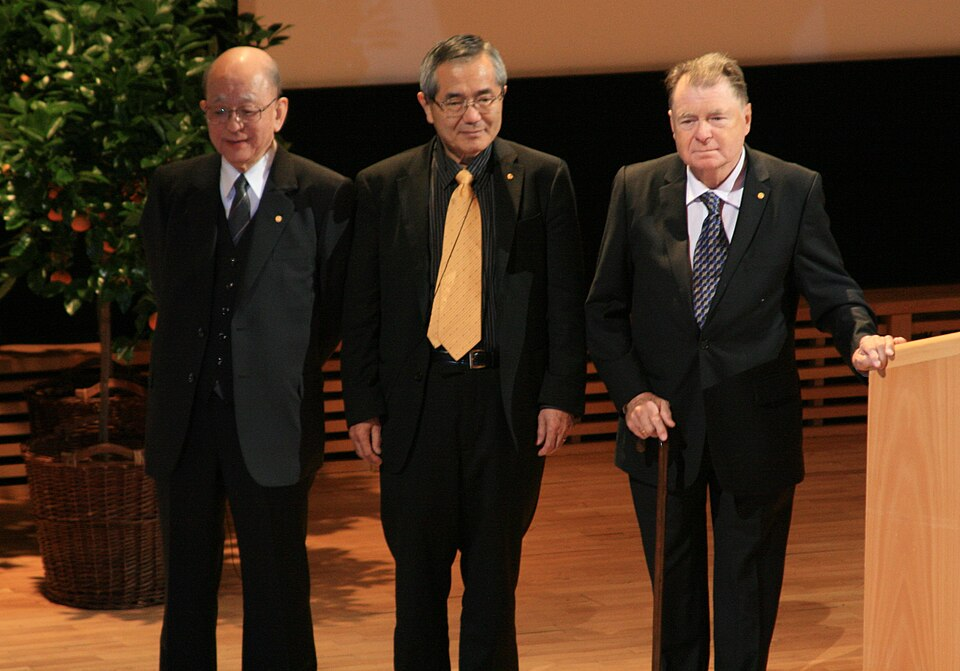
\includegraphics[width=\linewidth]{images/book3/nobel-2010.jpg}
\end{minipage}\hfill
\begin{minipage}[t]{0.6\linewidth}
\vspace{0pt}
ऐरिल और वाइनिल हैलाइडों के पैलेडियम-उत्प्रेरित युग्मनों ने --- ऐल्कीनों के साथ (रिचर्ड हेक,
1968 से), कार्बजस्ता अभिकर्मकों के साथ (एइइचि नेगिशी, 1977) और कार्बबोरॉन यौगिकों के साथ
(आकिरा सुज़ुकी, 1979) --- दो कार्बन ढाँचों को जोड़ना एक सामान्य काम बना दिया; ये अब औषधियों और पदार्थों के निर्माण में
सबसे अधिक प्रयुक्त अभिक्रियाओं में हैं। रसायन का नोबेल पुरस्कार
2010 में इन तीनों को दिया गया। (छायाचित्र: सुज़ुकी, नेगिशी और हेक, बाएँ
से दाएँ, 2010; ब्लडआइस, CC BY-SA 4.0, विकिमीडिया कॉमन्स।)
\end{minipage}
\end{history}

\begin{proposition}[आवर्त]\label{prop:b2:catalytic-cycles:tof}
यदि $n_P$ उत्पाद की वह मात्रा हो जो समय $t$ में उत्प्रेरक की मात्रा $n_{\text{उत्प्रेरक}}$ द्वारा बनती है,
तो $\mathrm{TON} = n_P/n_{\text{उत्प्रेरक}}$ और माध्य \omterm{def:b2:catalytic-cycles:cycle}{आवर्त आवृत्ति} $\mathrm{TOF} =
\mathrm{TON}/t$ है।
\end{proposition}

\begin{proof}
चक्र का हर चक्कर प्रति धातु परमाणु उत्पाद का एक अणु बनाता है; हर परमाणु द्वारा औसतन
किए गए चक्करों की संख्या $n_P/n_{\text{उत्प्रेरक}}$ है, और चक्कर लगाने की दर वह संख्या प्रति इकाई
समय है।
\end{proof}

\begin{safety}{\ghs[5mm]{GHS05}\,\ghs[5mm]{GHS07}\,\ghs[5mm]{GHS09}}
पैलेडियम(II) एथेनोएट आँखों के लिए संक्षारक और जलीय जीवों के लिए विषैला है;
ट्राइफ़ेनिलफ़ॉस्फ़ीन हानिकारक और संवेदीकारक है। इन्हें धूम-हुड में तौला जाता है, और
पैलेडियम के अवशेष पुनः प्राप्ति के लिए एकत्र किए जाते हैं, कभी नाली में नहीं बहाए जाते।
% ledger: ghs:Pd-acetate, ghs:PPh3, ghs:phenylboronic-acid, ghs:4-bromotoluene
\end{safety}

\section{अभ्यास}

\begin{exercise}[$\star$]\label{exo:b2:catalytic-cycles:1}
वास्का संकुल \ce{[IrCl(CO)(PPh3)2]} की ऑक्सीकरण अवस्था, $d^n$ और इलेक्ट्रॉन गणना दीजिए,
\ce{H2} जोड़ने से पहले और बाद में।
\end{exercise}

\begin{exercise}[$\star$]\label{exo:b2:catalytic-cycles:2}
चरण का नाम बताइए: \ce{[PtCl2(CH3)2(PR3)2] -> [PtCl2(PR3)2] + C2H6}; \ce{[Pd(Ph)Br(PR3)2] +
CH2=CH2 -> [Pd(CH2CH2Ph)Br(PR3)] + PR3}।
\end{exercise}

\begin{exercise}[$\star$]\label{exo:b2:catalytic-cycles:3}
कोई अभिक्रिया उत्प्रेरक के \qty{0.020}{mmol} का उपयोग करती है और
\qty{3.0}{h} में उत्पाद के \qty{15.0}{mmol} देती है। TON और माध्य TOF परिकलित कीजिए।
\end{exercise}

\begin{exercise}[$\star$]\label{exo:b2:catalytic-cycles:4}
सुज़ुकी चक्र के तीनों चरणों को जोड़िए और जाँचिए कि पैलेडियम कट जाता है।
\end{exercise}

\begin{exercise}[$\star\star$]\label{exo:b2:catalytic-cycles:5}
इनमें से कौन-से ऐल्किल पैलेडियम संकुल $\beta$-हाइड्राइड विलोपन कर सकते हैं:
\ce{Pd-CH3}, \ce{Pd-CH2CH3}, \ce{Pd-CH2C(CH3)3}, \ce{Pd-CH2Ph}, \ce{Pd-CH(CH3)2}?
\end{exercise}

\begin{exercise}[$\star\star$]\label{exo:b2:catalytic-cycles:6}
मेथिल प्रोपीनोएट के साथ आयडोबेन्ज़ीन की हेक अभिक्रिया के उत्पाद, और उसकी
ज्यामिति, का पूर्वानुमान कीजिए।
\end{exercise}

\begin{exercise}[$\star\star$]\label{exo:b2:catalytic-cycles:7}
प्रोपीन के हाइड्रोफ़ॉर्मिलन से बनने वाले रैखिक और शाखित ऐल्डिहाइड लिखिए, और
समझाइए कि कौन-सा निवेशन किस तक ले जाता है।
\end{exercise}

\begin{exercise}[$\star\star$]\label{exo:b2:catalytic-cycles:8}
\ce{[RhCl(PPh3)3]} एक फ़ॉस्फ़ीन खोने के बाद ही \ce{H2} क्यों जोड़ सकता है, जबकि
\ce{[RhCl(PPh3)2]} उसे तुरंत जोड़ लेता है?
\end{exercise}

\begin{exercise}[$\star\star$]\label{exo:b2:catalytic-cycles:9}
सुज़ुकी युग्मन में क्षारक क्यों आवश्यक है, और वह बोरोनिक अम्ल के साथ क्या करता है?
\end{exercise}

\begin{exercise}[$\star\star\star$]\label{exo:b2:catalytic-cycles:10}
किसी $d^8$ संकुल \ce{ML3X} (16 e) पर ऐल्कीन के हाइड्रोजनन के लिए प्रस्तावित एक चक्र
ऐल्कीन के बंधन से आरंभ होता है जो 20-इलेक्ट्रॉन संकुल देता है, फिर \ce{H2} का
\omterm{def:b2:catalytic-cycles:oxidative-addition}{ऑक्सीकारी योग}। त्रुटि खोजिए और क्रम ठीक कीजिए।
\end{exercise}

\begin{exercise}[$\star\star\star$]\label{exo:b2:catalytic-cycles:11}
किसी उत्प्रेरित अभिक्रिया के उत्पाद की मात्रा $n_P(t) = n_{\max}(1 - \mathrm e^{-t/\tau})$ के रूप में बढ़ती है,
जहाँ $n_{\max} = \qty{10.0}{mmol}$, $\tau = \qty{40}{min}$, और उत्प्रेरक \qty{0.010}{mmol} है
(अभ्यास के आँकड़े)। प्रारंभिक TOF और अंतिम TON परिकलित कीजिए।
\end{exercise}

\begin{exercise}[$\star\star\star$]\label{exo:b2:catalytic-cycles:12}
4-मेथॉक्सीबाइफ़ेनिल बनाने के लिए एक क्रॉस-युग्मन प्रस्तावित कीजिए, हैलाइड और बोरोनिक
अम्ल चुनते हुए, और चक्र लिखिए।
\end{exercise}

\section{समस्या: सुज़ुकी चक्र को पढ़ना}

\begin{problem}[{सप्ताहांत समस्या --- पूर्व-उत्प्रेरक और सक्रिय पैलेडियम(0),
किसी सुज़ुकी युग्मन का ऑक्सीकारी योग, पारधात्वन और अपचायी विलोपन,
लब्धि और आवर्त संख्या, और पार्श्व अभिक्रियाएँ}]
\label{pb:b2:catalytic-cycles:1}
प्रयोग (अभ्यास के आँकड़े): 4-ब्रोमोटॉलूईन के \qty{10.0}{mmol},
फ़ेनिलबोरोनिक अम्ल के \qty{12.0}{mmol}, पोटैशियम कार्बोनेट के \qty{20}{mmol}, पैलेडियम(II)
एथेनोएट के \qty{0.050}{mmol} और ट्राइफ़ेनिलफ़ॉस्फ़ीन के \qty{0.10}{mmol}, टॉलूईन, एथेनॉल और
जल के मिश्रण में, नाइट्रोजन के अंतर्गत गर्म किए गए; पृथक्कृत उत्पाद: 4-मेथिलबाइफ़ेनिल के \qty{1.51}{g}। मोलर
द्रव्यमान (\unit{g/mol}): 4-ब्रोमोटॉलूईन 171.04, फ़ेनिलबोरोनिक अम्ल 121.93, 4-मेथिलबाइफ़ेनिल
168.24, पैलेडियम(II) एथेनोएट 224.51।
% ledger: aw:C, aw:H, aw:Br, aw:B, aw:O, aw:Pd

\medskip
\noindent\textbf{भाग I --- उत्प्रेरक।}
\begin{enumerate}
  \item पैलेडियम(II) एथेनोएट में पैलेडियम की ऑक्सीकरण अवस्था और $d^n$ दीजिए।
  \item फ़्लास्क में यह \ce{Pd(PPh3)2} में अपचित होता है। इसकी ऑक्सीकरण अवस्था, $d^n$ और
        इलेक्ट्रॉन गणना दीजिए।
  \item वह संकुल उपसहसंयोजी रूप से असंतृप्त क्यों है?
  \item अभिक्रिया नाइट्रोजन के अंतर्गत क्यों चलाई जाती है?
  \item आधिक्य ट्राइफ़ेनिलफ़ॉस्फ़ीन की क्या भूमिका है?
  \item पैलेडियम(II) एथेनोएट उत्प्रेरक है या \omterm{def:b2:catalytic-cycles:cycle}{पूर्व-उत्प्रेरक}?
\end{enumerate}

\medskip
\noindent\textbf{भाग II --- चरण।}
\begin{enumerate}[resume]
  \item 4-ब्रोमोटॉलूईन का \omterm{def:b2:catalytic-cycles:oxidative-addition}{ऑक्सीकारी योग} लिखिए और उत्पाद की गणना कीजिए।
  \item कार्बोनेट फ़ेनिलबोरोनिक अम्ल के साथ क्या करता है?
  \item \omterm{def:b2:catalytic-cycles:transmetalation}{पारधात्वन} लिखिए।
  \item अगले चरण से पहले दोनों ऐरिल समूहों का cis होना क्यों आवश्यक है?
  \item \omterm{def:b2:catalytic-cycles:oxidative-addition}{अपचायी विलोपन} लिखिए और बनी पैलेडियम स्पीशीज़ की गणना कीजिए।
  \item तीनों चरणों को जोड़िए।
\end{enumerate}

\medskip
\noindent\textbf{भाग III --- लब्धि और आवर्त।}
\begin{enumerate}[resume]
  \item कौन-सा अभिकर्मक सीमांत है?
  \item पृथक्कृत उत्पाद की मात्रा परिकलित कीजिए।
  \item लब्धि परिकलित कीजिए।
  \item ब्रोमाइड के सापेक्ष mol~\% में उत्प्रेरक की मात्रा परिकलित कीजिए।
  \item पैलेडियम की \omterm{def:b2:catalytic-cycles:cycle}{आवर्त संख्या} परिकलित कीजिए।
  \item प्रयोग में \qty{4.0}{h} लगे। प्रति घंटा माध्य \omterm{def:b2:catalytic-cycles:cycle}{आवर्त आवृत्ति} परिकलित कीजिए।
\end{enumerate}

\medskip
\noindent\textbf{भाग IV --- पार्श्व अभिक्रियाएँ।}
\begin{enumerate}[resume]
  \item कुछ बाइफ़ेनिल \ce{Ph-Ph} मिलता है। सुझाइए कि यह कैसे बनता है।
  \item यहाँ कोई $\beta$-हाइड्राइड विलोपन संभव क्यों नहीं है?
  \item कोई ऐरिल क्लोराइड ब्रोमाइड की तुलना में बहुत धीमी अभिक्रिया करता है। कौन-सा चरण प्रभावित होता है?
  \item अभिक्रिया के अंत में पैलेडियम का क्या होता है, और उसे पुनः प्राप्त क्यों किया जाता है?
  \item बोरोनिक अम्ल का थोड़ा आधिक्य क्यों प्रयुक्त होता है?
  \item प्रयोग में पैलेडियम की \omterm{def:b2:catalytic-cycles:cycle}{आवर्त संख्या} बताइए।
\end{enumerate}
\end{problem}
